\chapter{MARCO TEÓRICO}
\section{Conceptos de ofuscación y código fuente}
\subsection{Lenguaje de programación}
``Los lenguajes de programación son notaciones que describen los cálculos a las personas y las máquinas. Nuestra percepción del mundo en que vivimos depende de los lenguajes de programación, ya que todo el software que se ejecuta en todas las computadoras se escribió en algún lenguaje de programación'' \cite[p. 1]{Aho2008}. Un lenguaje de programación es un lenguaje formal, que mediante un conjunto de instrucciones permite a un programador crear programas. El lenguaje de programación es un sistema estructurado de comunicación conformado por conjuntos de símbolos, palabras clave, reglas semánticas y sintácticas, las cuales sirven para el entendimiento entre un programador y una maquina.
\begin{itemize}
    \item \textbf{Palabra clave.} En los lenguajes de programacion existen palabras clave. Estas palabras no se pueden ser utilizadas para ningun otro proposito.
    \item \textbf{Funciones.} Tambien conocidos como subprogramas, procedimientos o metodos, las funciones son segmentos de codigo separado del bloque principal.
    \item \textbf{Tipos de datos.} En los lenguajes de programacion los tipos de datos son variados, los tipos de datos son atributos que indica la clase de dato que se va manejar. Los datos mas comunes son: Numeros enteros, numeros en coma flotante y cadenas.
    \item \textbf{Operadores.} Son simbolos que indican como manipular los operandos. Los operadores mas comunes son: Aritmeticos, relacionales, asignacion, logicos y tratamiento de bits.
    \item \textbf{Comentarios.} Son secuencias de caracteres que sirven para realizar anotaciones en el codigo fuente.
\end{itemize}

\subsection{Código fuente}
En informática, se denomina código fuente a la conjunto de lineas de texto que escritas por un programador. Estas lineas de texto representan instrucciones en un lenguaje de programación. Las instrucciones representan los pasos que debe seguir la computadora para la ejecución de un programa específico. El código fuente no es directamente ejecutable por la computadora, este debe ser traducido a otro lenguaje de modo que la computadora pueda interpretarlo. En la traducción se usan compiladores, ensambladores, interpretes y otros.

\subsection{Ofuscación de código fuente}
En computación, la ofuscación de código fuente se refiere al acto de realizar cambios no destructivos en código fuente de un programa. Es decir, se alteran las instrucciones del código fuente manteniendo su funcionamiento original, la ofuscación de un programa se realiza para dificultar su entendimiento, también puede ser utilizado para ocultar la similitud con el programa original. Un ejemplo se muestra en la figura \ref{obfuscationSC}.


\begin{figure}[!h]
\centering
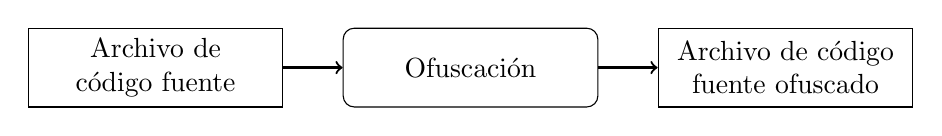
\begin{tikzpicture}[scale=1,
input_output/.style ={rectangle, minimum width=1cm, minimum height=1cm,text centered, text width=3cm, draw=black},
algorithm/.style={rectangle, rounded corners, minimum width=3cm, minimum height=1cm,text centered, text width=3cm, draw=black},
arrow/.style={thick,->,},
]
\node[input_output] (n0) at (1,1) {Archivo de código fuente};
\node[algorithm] (n1) at (5,1) {Ofuscación};
\node[input_output] (n2) at (9,1) {Archivo de código fuente ofuscado};
\draw [arrow] (n0.east) to (n1.west);
\draw [arrow] (n1.east) to (n2.west);
\end{tikzpicture}
\caption{Ofuscación de código fuente}
Fuente: Elaboración propia.
\label{obfuscationSC}
\end{figure}


Una definición formal se encuentra en \cite{Collberg1997} que define a la ofuscación de código fuente de la siguiente manera: Dado un programa $P$, y el programa transformado ${P}'$. Se define a $T$ como la transformación de ofuscación como $P\overset{T}{\rightarrow}{P}'$, donde requiere que $P$ y ${P}'$ mantengan el mismo comportamiento observacional, Ademas si $P$ no puede terminar o termina con errores, entonces ${P}'$ puede terminar o no, y ${P}'$ debe terminar si ${P}$ termina.

\subsection{Métodos de ofuscación de código fuente}
\cite{Novak2019} Explica que existen muchos métodos de ofuscación son utilizados para ocultar la similitud, a su vez menciona que en un estudio de 72 artículos se identificaron 25 métodos de ofuscación, y de estos se especificaron 16 métodos distintos. Existen muchos métodos para la ofuscación, a continuación se presentan los métodos mas importantes, cada método tiene su ejemplo de ofuscación en el lenguaje de programacion Python.

\begin{itemize}
    \item \cite{article3} Mencionan cambios en el formato del código. Como la agregación o eliminación de: Espacios en blanco, sangrías y saltos de linea. El ejemplo se muestra en los programas \ref{lst:obfuscation1_1} y \ref{lst:obfuscation1_2}.
    \lstinputlisting[caption={Cambio del formato del código, original},label={lst:obfuscation1_1}, language=Python]{programs/obfuscation/obfuscation1_1.py}
    \lstinputlisting[caption={Cambio del formato del código, modificado},label={lst:obfuscation1_2}, language=Python]{programs/obfuscation/obfuscation1_2.py}

    \item \cite{article3} Mencionan cambios en los comentarios del código. Como la agregación, modificación o eliminación de los comentarios. El ejemplo se muestra en los programas \ref{lst:obfuscation2_1} y \ref{lst:obfuscation2_2}.
    \lstinputlisting[caption={Cambios de comentarios, original},label={lst:obfuscation2_1}, language=Python]{programs/obfuscation/obfuscation2_1.py}
    \lstinputlisting[caption={Cambios de comentarios, modificado},label={lst:obfuscation2_2}, language=Python]{programs/obfuscation/obfuscation2_2.py}

    \item \cite{Zoran2012} y \cite{donaldson1981plagiarism} Mencionan el cambio de los nombres de los identificadores. Es decir, cambios en los nombres de variables, nombres de constantes, nombres de funciones, nombres de clases, etc. El ejemplo se  muestra en los programas \ref{lst:obfuscation3_1} y \ref{lst:obfuscation3_2}.
    \lstinputlisting[caption={Cambio en los nombres de las variables, original},label={lst:obfuscation3_1}, language=Python]{programs/obfuscation/obfuscation3_1.py}
    \lstinputlisting[caption={Cambio en los nombres de las variables, modificado},label={lst:obfuscation3_2}, language=Python]{programs/obfuscation/obfuscation3_2.py}

    \item \cite{donaldson1981plagiarism} Menciona cambios en el orden en las declaraciones de las variables. El ejemplo se muestra en los programas \ref{lst:obfuscation4_1} y \ref{lst:obfuscation4_2}.
    \lstinputlisting[caption={Cambio en el orden de declaraciones de variables, original},label={lst:obfuscation4_1}, language=Python]{programs/obfuscation/obfuscation4_1.py}
    \lstinputlisting[caption={Cambio en el orden de declaraciones de variables, modificado},label={lst:obfuscation4_2}, language=Python]{programs/obfuscation/obfuscation4_2.py}

    \item \cite{Grier1981} Menciona agregar lineas de código innecesarias. El ejemplo se muestra en los programas \ref{lst:obfuscation5_1} y \ref{lst:obfuscation5_2}.
    \lstinputlisting[caption={Agregar instrucciones innecesarias, original},label={lst:obfuscation5_1}, language=Python]{programs/obfuscation/obfuscation5_1.py}
    \lstinputlisting[caption={Agregar instrucciones innecesarias, modificado},label={lst:obfuscation5_2}, language=Python]{programs/obfuscation/obfuscation5_2.py}

    \item \cite{WHALE1990131} Menciona el reemplazo de la llamada de un procedimiento por el procedimiento. El ejemplo se muestra en los programas \ref{lst:obfuscation6_1} y \ref{lst:obfuscation6_2}.
    \lstinputlisting[caption={Reemplazo de la llamada a un procedimiento, original},label={lst:obfuscation6_1}, language=Python]{programs/obfuscation/obfuscation6_1.py}
    \lstinputlisting[caption={Reemplazo de la llamada a un procedimiento, modificado},label={lst:obfuscation6_2}, language=Python]{programs/obfuscation/obfuscation6_2.py}

    \item \cite{WHALE1990131} Menciona el cambio de la especificación de una declaración. Cambios como: El cambio de las operaciones y el operando, cambio en los tipos de datos. El ejemplo se muestra en los programas \ref{lst:obfuscation7_1} y \ref{lst:obfuscation7_2}.
    \lstinputlisting[caption={Cambio de operaciones y operandos, original},label={lst:obfuscation7_1}, language=Python]{programs/obfuscation/obfuscation7_1.py}
    \lstinputlisting[caption={Cambio de operaciones y operandos, modificado},label={lst:obfuscation7_2}, language=Python]{programs/obfuscation/obfuscation7_2.py}

    \item \cite{article3} Mencionan el cambio de estructuras de control por sus equivalentes. El reemplazo por equivalentes de estructuras repetitivas y condicionales, El ejemplo se muestra en los programas \ref{lst:obfuscation8_1} y \ref{lst:obfuscation8_2}.
    \lstinputlisting[caption={Cambio en la estructura repetitiva, original},label={lst:obfuscation8_1}, language=Python]{programs/obfuscation/obfuscation8_1.py}
    \lstinputlisting[caption={Cambio en la estructura repetitiva, modificado},label={lst:obfuscation8_2}, language=Python]{programs/obfuscation/obfuscation8_2.py}
\end{itemize}

\cite{Bejarano2015} se refiere a los métodos como modificaciones y los divide en dos grupos:
\begin{itemize}
  \item \textbf{Cambios léxicos}. Estos no requieren un análisis gramatical o profundo conocimiento de programación para ser eficaces. Algunos ejemplos son: Eliminar comentarios, cambiar el formato de código fuente y cambiar los nombres de las variables.
  \item \textbf{Cambios estructurales}. Estos requiere conocimiento acerca de los lenguajes y técnicas de programación, estos cambios son altamente dependiente de el lenguaje de programación. Algunos ejemplos son: cambiar las estructuras de control, cambiar el orden de las sentencias, reemplazar la llamada a un procedimiento por el procedimiento, etc.
\end{itemize}

\subsection{Niveles de transformación}
Una de las investigación mas antiguas respecto a la ofuscación de código fuente, fue desarrollado por \cite{Faidhi1987} en su trabajo se refiere a los métodos utilizados para las ofuscación como transformaciones para ocultar la similitud. Explica que las transformaciones pueden ser divididas en niveles. Donde en niveles bajos se encuentran las transformaciones que realiza un programador novato para ocultar la similitud, y los niveles altos se encuentran las transformaciones que realiza un programador experto para ocultar la similitud. A continuación el detalle de estos niveles de transformación.
\begin{itemize}
  \item \textbf{Nivel 1.} Representa los cambios en los comentarios e indentación.
  \item \textbf{Nivel 2.} Representa cambios de nivel 1, y cambios en los identificadores.
  \item \textbf{Nivel 3.} Representa cambios de nivel 2, y cambios en las declaraciones. Es decir declarar constantes extras, cambiar las posiciones de las variables declaradas.
  \item \textbf{Nivel 4.} Representa cambios de nivel 3, y modificación de los métodos. Es decir cambios en las asignaciones de la funciones, cambiar de funciones por procedimientos, combinar y crear nuevas funciones.
  \item \textbf{Nivel 5.} Representa cambios de nivel 4. y cambios en las sentencias equivalentes. Es decir cambios en las estructuras de control equivalentes un for por un while.
  \item \textbf{Nivel 6.} Representa cambios de nivel 5, y cambios en las decisiones lógica. Es decir cambios en la expresiones.
\end{itemize}

\section{Detección de similitud de código fuente}
\cite{Novak2019} Realizo un estudio sistemático campo de la detección de plagio de código fuente, describe definiciones de plagio, herramientas para la detección de plagio, métricas de comparación, métodos de ofuscación, conjunto de datos para la comparación y algoritmos que utilizan las herramientas.
\subsection{Clasificacion de algoritmos para la detección de similitud}
En su estudio \cite{Novak2019} identifica algoritmos basados en estilo, basado en semántica, basado en texto, huellas dactilares, recuento de atributos, basado en estructura, coincidencia de cadenas, marca de agua, basado en historial, basado en XML, código compilado, basado en compresión, basado en grafos, basado en agrupamiento, basado en N-gramas y basado en árboles. También hace menciona que los enfoques basados en estructuras son mucho mejores y que la mayoría de las herramientas combinan más de un tipo de algoritmo. En el cuadro \ref{tiposDeAlgoritmos} se muestra detalles de estos como el primer y ultimo año de publicación de un algoritmo, el numero de artículos en los que aparecen y si utilizan la tokenización.

\begin{table}[H]
\centering
\begin{tabular}{|lllll|}
\hline
\multicolumn{1}{|c|}{Tipo de algoritmo}       & \multicolumn{1}{c|}{Ultimo año} & \multicolumn{1}{c|}{Primer año} & \multicolumn{1}{c|}{Nro. de artículos} & \multicolumn{1}{c|}{Tokenización} \\ \hline\hline
\multicolumn{1}{|l|}{Basado en estilo}        & \multicolumn{1}{c|}{2016}       & \multicolumn{1}{c|}{2011}       & \multicolumn{1}{c|}{5}                 & \multicolumn{1}{c|}{2}           \\ \hline
\multicolumn{1}{|l|}{Basado en semántica}     & \multicolumn{1}{c|}{2013}       & \multicolumn{1}{c|}{2010}       & \multicolumn{1}{c|}{7}                 & \multicolumn{1}{c|}{5}            \\ \hline
\multicolumn{1}{|l|}{Basado en texto}         & \multicolumn{1}{c|}{2016}       & \multicolumn{1}{c|}{1996}       & \multicolumn{1}{c|}{9}                 & \multicolumn{1}{c|}{5}           \\ \hline
\multicolumn{1}{|l|}{Huellas dactilares}      & \multicolumn{1}{c|}{2015}       & \multicolumn{1}{c|}{2005}       & \multicolumn{1}{c|}{11}                & \multicolumn{1}{c|}{4}            \\ \hline
\multicolumn{1}{|l|}{Recuento de atributos}   & \multicolumn{1}{c|}{2015}       & \multicolumn{1}{c|}{1980}       & \multicolumn{1}{c|}{25}                & \multicolumn{1}{c|}{6}            \\ \hline
\multicolumn{1}{|l|}{Basado en estructura}    & \multicolumn{1}{c|}{2016}       & \multicolumn{1}{c|}{1980}       & \multicolumn{1}{c|}{25}                & \multicolumn{1}{c|}{13}           \\ \hline
\multicolumn{1}{|l|}{Coincidencia de cadenas} & \multicolumn{1}{c|}{2016}       & \multicolumn{1}{c|}{1981}       & \multicolumn{1}{c|}{26}                & \multicolumn{1}{c|}{17}           \\ \hline\hline
\multicolumn{5}{|c|}{Nuevas categorías identificadas}                                                                                                                    \\ \hline\hline
\multicolumn{1}{|l|}{Marca de agua}           & \multicolumn{1}{c|}{2013}       & \multicolumn{1}{c|}{2005}       & \multicolumn{1}{c|}{2}                 & \multicolumn{1}{c|}{0}            \\ \hline
\multicolumn{1}{|l|}{Basado en historial}     & \multicolumn{1}{c|}{2016}       & \multicolumn{1}{c|}{2013}       & \multicolumn{1}{c|}{2}                 & \multicolumn{1}{c|}{0}            \\ \hline
\multicolumn{1}{|l|}{Basado en XML}           & \multicolumn{1}{c|}{2012}       & \multicolumn{1}{c|}{2010}       & \multicolumn{1}{c|}{3}                 & \multicolumn{1}{c|}{2}            \\ \hline
\multicolumn{1}{|l|}{Código compilado}        & \multicolumn{1}{c|}{2015}       & \multicolumn{1}{c|}{2006}       & \multicolumn{1}{c|}{5}                 & \multicolumn{1}{c|}{2}            \\ \hline
\multicolumn{1}{|l|}{Basado en compresión}    & \multicolumn{1}{c|}{2010}       & \multicolumn{1}{c|}{2004}       & \multicolumn{1}{c|}{6}                 & \multicolumn{1}{c|}{5}            \\ \hline
\multicolumn{1}{|l|}{Basado en grafos}        & \multicolumn{1}{c|}{2015}       & \multicolumn{1}{c|}{2005}       & \multicolumn{1}{c|}{10}                & \multicolumn{1}{c|}{2}            \\ \hline
\multicolumn{1}{|l|}{Basado en agrupamiento}  & \multicolumn{1}{c|}{2015}       & \multicolumn{1}{c|}{2005}       & \multicolumn{1}{c|}{11}                & \multicolumn{1}{c|}{7}            \\ \hline
\multicolumn{1}{|l|}{Basado en N-gramas}      & \multicolumn{1}{c|}{2016}       & \multicolumn{1}{c|}{2006}       & \multicolumn{1}{c|}{15}                & \multicolumn{1}{c|}{9}            \\ \hline
\multicolumn{1}{|l|}{Basado en árboles}       & \multicolumn{1}{c|}{2015}       & \multicolumn{1}{c|}{1988}       & \multicolumn{1}{c|}{24}                & \multicolumn{1}{c|}{8}            \\ \hline
\end{tabular}
\caption{Descripción general de los tipos de algoritmos}
Fuente: \cite{Novak2019}.
\label{tiposDeAlgoritmos}
\end{table}


\cite{Novak2019} Menciona que las tres herramientas principales para la detección de similitud, utilizan los algoritmos de Running-Karp-Rabin Greedy-String-Tiling (RKRGST), Winnowing-Fingerprint (W-F) e implementaciones de tokenización.

\subsection{Técnicas para la detección de similitud}
En su investigación \cite{Karnalim2019} clasifica las técnicas de detección de similitud en tres categorías: Basadas en conteo de atributos, basadas en estructuras y técnicas híbridas, a continuación se dará una breve descripción de cada una de ellas.

\begin{enumerate}
    \item \textbf{Técnicas basadas en conteo de atributos}. Estas técnicas determinan la similitud comparando las frecuencias de ocurrencias de los atributos del código fuente.
    \begin{enumerate}
      \item \textbf{Técnica estándar de conteo de atributos}. Esta técnica considera similares a dos archivos de código fuente si sus frecuencias de ocurrencias de sus atributos son las mismas. Como los operandos, operadores, espacios en blanco, numero de lineas, comentarios, declaraciones y otros. Uno de los primeros trabajos presentados fue por \cite{Ottenstein1976} en el cual utiliza cuatro métricas de software: El numero de operadores únicos, operandos únicos, operadores y operandos.
      \item \textbf{Técnicas basadas en recuperación de información}. Esta técnica se basa en realizar consultas especificas a una gran colección de documentos, Una consulta especifica es un segmento de código o archivo y la colección de documentos son los archivos cuyo contenido es similar al segmento o archivo inicial. Las técnicas basadas en recuperacion de la información (IR) se basan en el análisis semántico latente (LSA), y tiene como objetivo encontrar relaciones entre términos con la ayuda de descomposición en valores singulares. \cite{Cosma2012} utilizaron LSA para detectar similitud en trabajos realizados por estudiantes obteniendo buenos resultados, sugiriendo que la técnica puede mejorar el rendimiento en las herramientas de detección existente como JPLAG y Sherlock.
      \item \textbf{Técnicas basadas en agrupamiento}. En esta técnica los archivos de código fuente similares se muestran en grupos. \cite{Moussiades2005} fue el primero en utilizar la técnica que consiste en convertir los archivos en tokens y luego los agrupa utilizando un algoritmo de agrupación.
      \item \textbf{Técnicas basadas en clasificación}. Esta técnica aprende a buscar patrones de similitud de código fuente. \cite{Yasaswi2017} utilizo su algoritmo de clasificación para detectar la similitud ponderando las características, según el modelo de un lenguaje a nivel de caracteres, el cual se entreno en el código fuente del kernel de Linux.
      \item \textbf{Técnicas combinadas con conteo de atributos}. Varias técnicas de conteo de atributos se combinan con otras técnicas para mejorar la detección. En su trabajo \cite{Sidorov2017} combina técnicas basadas en recuperacion de información y clasificación, su técnica consiste en convertir los archivos en tokens de N-gramas sobre los cuales se realizara el análisis semántico latente.
    \end{enumerate}
    \item \textbf{Técnicas basadas en estructuras}. Estas técnicas comparan estructuras de dos códigos fuente para determinar su similitud.
    \begin{enumerate}
      \item \textbf{Técnicas basadas en emparejamiento de cadenas}. Esta técnica es de las mas antiguas y populares, En su investigación \cite{Wise1992} compara dos archivos de código fuente convirtiéndolos en cadenas de tokens, y para la medición de similitud usa el comando sdiff de UNIX.
      \item \textbf{Técnicas basadas en emparejamiento de arboles y grafos}. La comparación de arboles o grafos puede llegar a tomar un tiempo considerable, por lo cual esta técnica suele incorporar simplificaciones que reduzcan el tiempo. En su investigación \cite{Song2015} calcula la similitud de código fuente de dos programas. Utilizando la información sintáctica del código fuente expresado como un árbol de análisis, la similitud sintáctica entre dos programas se calcula mediante un núcleo de árbol de análisis.
    \end{enumerate}
    \item \textbf{Técnicas híbridas} Estas técnicas combinan las técnicas de recuento de atributos, técnicas basadas en estructuras y otras. con el fin de mejorar la eficacia y eficiencia, para la comparación de similitud entre códigos fuente.
\end{enumerate}

\subsection{Herramientas para la detección de similitud}

\cite{Novak2019} describe cuatro características de cinco herramientas que son consideradas las más importantes, en el cuadro \ref{descripcionHerramientas} se muestran las características como: las menciones en artículos, código abierto, interfaz grafica (GUI), sin conexión a internet y el sitio web.

\begin{table}[H]
\centering
\begin{tabular}{|c||c|c|c|c|c|}
\hline
Herramienta      & Menciones & Código abierto & GUI & offline & Sitio web \\ \hline\hline
JPLAG        & 43                & Si             & Si  & Si                      & \href{https://jplag.ipd.kit.edu}{jplag.ipd.kit.edu} \\ \hline
MOSS          & 38                & No             & Si  & No                      & \href{https://theory.stanford.edu/~aiken/moss/}{theory.stanford.edu} \\ \hline
Sherlock & 9                 & Si             & Si  & Si                      & \href{http://warwick.ac.uk/iasgroup/software/sherlock}{warwick.ac.uk}  \\ \hline
Plaggie             & 7                 & Si             & Si  & Si                      &  \href{https://www.cs.hut.fi/Software/Plaggie}{www.cs.hut.fi} \\ \hline
SIM            & 6                 & Si             & No  & Si                      &  \href{https://dickgrune.com/Programs/similary_tester}{dickgrune.com} \\ \hline
\end{tabular}
\caption{Descripción general de las características de las herramientas}
Fuente: \cite{Novak2019}.
\label{descripcionHerramientas}
\end{table}


\cite{Ragkhitwetsagul2018} Realizo un estudio sobre métodos y herramientas para la detección de similitud, en el cual identifica las medidas de similitud que utilizan las cinco herramientas mas populares. En el cuadro \ref{descripcionHerramientasMedida} se muestra los detalles de las medidas de similitud que utilizan las cinco herramientas más populares.

\begin{table}[H]
\centering
\begin{tabular}{|r||l|}
\hline
Herramientas & Medida de similitud utilizadas \\ \hline\hline
JPLAG       & Tokens y Greedy-String-Tiling \\ \hline
MOSS        & Winnowing-Fingerprint \\ \hline
Sherlock    & Firmas Digitales  \\ \hline
Plaggie     & Token-Tiling  \\ \hline
SIM         & Alineamiento de cadenas  \\ \hline
\end{tabular}
\caption{Herramientas con sus medidas de similitud}
Fuente: \cite{Ragkhitwetsagul2018}.
\label{descripcionHerramientasMedida}
\end{table}


\subsubsection{JPLAG}
\cite{Prechelt2003} Explica que JPLAG es un servicio web que encuentra programas similares entre un conjunto de programas. Se ha utilizado con éxito para detectar plagio entre los envíos de programas Java de los estudiantes. Está disponible para los lenguajes C, C++ y Scheme, su algoritmo de comparación, se basa en uno conocido como Running-Rabin-Karp Greedy-String-Tiling. \cite{Cheers2021} Explica que JPLAG opera aplicando un algoritmo Token-Tiling para cubrir un archivo de código fuente con tokens extraídos de otro. Si dos archivos fuente tienen un alto grado de cobertura, pueden considerarse similares y, por lo tanto, candidatos a plagio. Primero, los archivos de código fuente se convierten en un flujo de tokens. JPlag utiliza su propio conjunto de tokens que abstraen los tokens de lenguaje estándar para evitar hacer coincidir el mismo token con diferentes significados. En segundo lugar, los tokens extraídos se comparan entre archivos para determinar la similitud mediante el algoritmo Running-Karp-Rabin Greedy-String-Tiling, donde los tokens de un archivo se superponen a los de otro dentro de una tolerancia de desajuste. La similitud del programa se evalúa como el porcentaje de tokens de un programa que se pueden colocar sobre otro programa.
\subsubsection{MOSS}
\cite{Hage2010} Explica que MOSS es un Software creado por el profesor Alex Aiken en la universidad de Stanford, siendo el primer servicio que inició en la web, una referencia a nivel mundial. MOSS permite comparar hasta 250 archivos en 25 lenguajes de programación. \cite{Pachon2019} Explica que MOSS no tiene licencia como software libre, el uso de MOSS dentro del ambiente académico es gratuito y ofrecido desde un servidor de Stanford. Es difícil su configuración y tiene poca documentación.
\subsubsection{Sherlock}
\cite{Cheers2021} Explica que Sherlock implementa métodos de comparación de texto y tokenizados. En la herramienta, se compara la similitud de un par de programas 5 veces: en su forma original, se eliminan los espacios en blanco y los comentarios, como un archivo fuente tokenizado. En todos los casos, las comparaciones miden la similitud a través de la identificación de ejecuciones, una secuencia de líneas comunes a dos archivos que pueden verse interrumpidas por anomalías, como líneas adicionales.

\subsubsection{Plaggie}
 \cite{Ahtiainen2006} Explica que Plaggie es una aplicación Java independiente que se puede utilizar para comprobar ejercicios de programación Java. La funcionalidad de Plaggie es similar al servicio web JPlag publicado anteriormente, pero a diferencia de JPlag, Plaggie debe instalarse localmente y su código fuente está abierto. Aparentemente, Plaggie es el único motor de detección de plagio de código abierto para ejercicios de Java. \cite{Cheers2021} Explica que Plaggie es una herramienta que se afirma que funciona de manera similar a JPlag. Plaggie es una aplicación local en comparación con JPlag que originalmente se proporcionó como un servicio web, no existe una publicación que describa el funcionamiento de Plaggie, sin embargo, al examinar su código fuente, opera sobre representaciones tokenizadas de código que evalúan la similitud mediante Token-Tiling.
\subsubsection{SIM}
\cite{Cheers2021} Explica que SIM analiza programas en busca de similitud estructural mediante el uso de alineación de cadenas. Para dos programas, SIM primero analiza el código fuente creando un árbol de análisis. Luego, la herramienta representará los árboles de análisis como cadenas y los alineará insertando espacios para obtener una subsecuencia común máxima de sus tokens contenidos. La similitud de los programas se evalúa luego como el número de coincidencias.

%\section{Algoritmos para la deteccion de similitud}
%\subsection{Algoritmo Greedy-String-Tiling}
%\subsection{Algoritmo Winnowing-Fingerprint}

\section{Indices de similitud}
\cite{magurran1988} explica que los indices de similitud expresan el grado en que dos muestras son semejantes por las especies presentes en ellas. Estos valores pueden obtenerse con base en datos cualitativos o cuantitativos.

\subsection{Indice de Sorensen-Dice}
El indice de Sorensen-Dice también conocido como el coeficiente de Sorencen. Es un estadístico utilizado para comparar la similitud entre dos muestras. El indice de Sorencen-Dice se define como:

\begin{equation}
S = \frac{2*|A \cap B|}{|A|+|B|}
\label{sorencen}
\end{equation}

En la ecuacion \ref{sorencen} se muestra a: $|\id{A}|$ y $|\id{B}|$ como el numero de especies en las muestras \id{A} y \id{B}, $|A \cap B|$ como el numero de especies compartidas por las muestras y \id{S} como el indice de similitud y varia entre 0 a 1. Es decir se encuentra en el rango de $[0 \twodots 1]$.

\subsection{Indice de Jaccard}
El indice de Jaccard tambien conocido como el coeficiente de Jaccard, Es un estadistico utilizado para medir el grado de similitud entre dos conjuntos. El indice de Jaccard se define como:
\begin{equation}
J = \frac{|A \cap B|}{|A \cup B|}
\label{jaccard}
\end{equation}
En la ecuacion \ref{jaccard} se muestra a: $|A \cup B|$ como el numero de especies en las muestras \id{A} y \id{B}, $|A \cap B|$ como el numero de especies compartidas por las muestras y \id{J} como el indice de similitud y varia entre 0 a 1. Es decir se encuentra en el rango de $[0 \twodots 1]$.

\section{Conceptos de compiladores y tokens}
\subsection{Procesador de lenguaje}
Un procesador de lenguaje también llamado compilador. \cite{Aho2008} Explica que un procesador de lenguaje es un programa que puede leer un programa en un lenguaje y traducirlo en un programa equivalente en otro lenguaje. Una función importante del compilador es reportar cualquier error en el programa fuente que detecte durante el proceso de traducción.

\subsection{Análisis Léxico}
Una analizador lexico tambien es conocido como Lexer. \cite{Aho2008} Explica que la primera fase de un procesador de lenguaje, se le llama análisis léxico o escaneo. El analizador léxico lee el flujo de caracteres que componen el programa fuente y los agrupa en secuencias significativas, conocidas como lexemas. Para cada lexema, el analizador léxico produce como salida un token. Estos lexemas son los que pasaran a la siguiente fase, el análisis de la sintaxis. El analizador léxico ignora los espacios en blanco que separan los lexemas. \cite{catalan2010compiladores} Explica que esta fase consiste en leer el texto del código fuente carácter a carácter e ir generando los tokens. Estos tokens constituyen la entrada para el siguiente proceso de análisis. El agrupamiento de caracteres en tokens depende del lenguaje que se va a compilar. Es decir un lenguaje generalmente agrupara caracteres en tokens diferentes de otro lenguaje. Los tokens pueden ser de dos tipos, cadenas específicas como palabras reservadas, puntos y comas, etc., y no específicas, como identificadores, constantes y etiquetas. La diferencia entre ambos tipos de tokens radica en si ya son conocidos previamente o no. El analizador léxico irá ignorando las partes no esenciales para la siguiente fase, como pueden ser los espacios en blanco, los comentarios, etc., es decir, realiza la función de preprocesador en cierta medida. Por lo tanto, y resumiendo, el analizador léxico lee los caracteres que componen el texto del programa fuente y suministra tokens al analizador sintáctico.

\subsection{Tokenización de codigo fuente}
Los tokens son la unidad léxica basica, y los lexemas son las palabras de un codigo fuente. \cite{Aho2008} Explica los pasos para generar un token. Primeramente se leen los lexemas que componen del código fuente y los agrupa en categorías según su función, este proceso es llamado tokenización. En un lenguaje de programación un token puede tener en clases como: constantes, identificadores, operadores, palabras reservadas y separadores. Por ejemplo, suponga que un código fuente contiene la instrucción de asignación: $\id{posicion = inicial + velocidad * 60}$. En este ejemplo se ignora los espacios en blanco que separan a los lexemas, y los nombres de los lexemas =, + y * serán considerados como símbolos abstractos. A continuación se muestra el detalle de la tokenización de la instrucción:
\begin{itemize}
    \item $\id{posicion}$: es un lexema, se le asigna al token $[\id{id}, 1]$, en donde $\id{id}$ es un símbolo abstracto que representa la palabra identificador y 1 apunta a la entrada en la tabla de símbolos para $\id{posicion}$. La entrada en la tabla de símbolos para un identificador contiene información acerca de éste, como su nombre y tipo.
    \item $=$: El símbolo de asignación es un lexema, se al asigna el token $[=]$. Como este token no necesita un valor-atributo, se omite el segundo componente.
    \item $\id{inicial}$: es un lexema, se le asigna al token $[id, 2]$, en donde 2 apunta a la entrada en la tabla de símbolos para $\id{inicial}$.
    \item $+$: es un lexema, se le asigna al token $[+]$.
    \item $\id{velocidad}$: es un lexema, se le asigna al token $[id, 3]$, en donde 3 apunta a la entrada en la tabla de símbolos para $\id{velocidad}$.
    \item $*$: es un lexema, se le asigna al token $[*]$.
    \item $60$: es un lexema, se le asigna al token $[60]$.
\end{itemize}

\noindent Finalmente se obtiene los siguientes tokens: $[id, 1] [=] [id, 2] [+] [id, 3] [*] [60]$.

\section{Conceptos de programacion dinamica y distancia de edicion}
\subsection{Programación dinámica}
\cite{Cormen2009} Explica que la programación dinámica es un método para la resolución de problemas, el cual resuelve un problema combinando las soluciones de los subproblemas. La programación dinámica se aplica cuando los problemas se superponen, cuando los subproblemas comparten subproblemas, donde un algoritmo de programación dinámica resuelve un subproblemas solo una vez y guarda la respuesta en una tabla, de esta forma evita el trabajo de volver a calcular la respuesta. La programación dinámica se aplica a problema de optimización dichos problemas pueden tener mas de una solución posible, en el cual se desea encontrar el máximo o mínimo, a estas soluciones se llaman solución optima.\\

\noindent Para desarrollar un algoritmo de programación de dinámica se sigue la siguiente secuencia de pasos:
\begin{enumerate}
    \item Caracterizar la estructura de solución optima.
    \item Definir recursivamente el valor de una solución optima.
    \item Calcular el valor de una solución optima, normalmente en forma ascendente.
    \item Construir una solución optima a partir de la información calculada.
\end{enumerate}

\subsection{El problema de la distancia de edicion}
\cite{Cormen2009} explica que el problema de la alineación de cadenas o distancia de edición, consiste en dadas dos cadenas $A=[1 \twodots n]$ y $B=[1 \twodots m]$, y un conjunto de operaciones de transformación y sus costos. La distancia de edición de $A$ a $B$ es el costo de la secuencia de operaciones menos costosa que transforma $A$ en $B$, las operaciones se realizan en los caracteres de la cadena. La distancia de edición es una forma de medir que tan diferentes son dos cadenas entre si.

\subsection{Tipos de distancia de edicion}
\cite{Navarro2001} explica que existen diferentes tipos de distancia de edicion, las cuales se distinguen al permitir diferentes operaciones en las cadenas.
\begin{itemize}
  \item La distancia de la subsecuencia comun mas larga, permite la inserción y eliminacion.
  \item La distancia de Levenshtein, permite la eliminacion, inserción y reemplazamiento.
  \item La distancia de Damerau-Levenshtein, permite la insercion, eliminacion, reemplazamiento y transposicion de dos caracteres adyacentes.
\end{itemize}
Las primeras referencias de este problema son de los años sesenta y setenta, donde el problema de la distancia de edicion aparece en diferentes campos. En el campo de la biologia computacional, procesamiento de señales y recuperacion de texto. En la biologia computacional, las secuencias de ADN y proteinas se ven como textos extensos sobre alfabetos, estas secuencias representan el codigo genetico de los seres vivos. Por lo cual encontrar secuencias especificas sobre estos textos, son operaciones fundamentales para problemas como el ensamblaje de la cadena del ADN o la deteminacion de que tan diferentes son dos secuencias geneticas. Todo esto se modela como la busqueda de patrones en un texto, como ejemplo se tiene el algoritmo de programacion dinamica de Needleman-Wunsch que resuelve el problema de la alineación global de secuenciasde ADN. En el campo del procesamiento de señales, uno de los problemas es la correccion de errores de transmision. La transmision fisica de señales es propensa a errores, de modo que para asegurar una transmision correcta a travez de un canal fisico, es necesario ser capaz de recuperar el mensaje correcto despues de una posible modificacion introducida durante la transmision. Dado que la modificacion no es conocida se requiere un texto que este mas cercano al mensaje enviado, como ejemplo se tienen algoritmos de programacion dinamica que resuelve el problema de la distancia de Levenshtein. En el campo de la recuperacion de texto, tiene como problema principal la correccion de errores de ortograficos de un texto. Esta es una de las aplicaciones antiguas con mas potencial, como ejemplo se tienen algoritmos de programacion dinamica que resuelven el problema de la distancia de Damerau-Levenshtein que permite transposicion de caracteres adyacentes.

\section{La distancia de la subsecuencia comun mas larga}
La subsecuencia comun mas larga tambien es conocida por sus siglas en ingles como \id{LCS}. En \cite{Cormen2009} encontramos las siguientes definiciones. Dada una secuencia $\id{X} = [x_1, x_2, \twodots, x_m]$, una secuencia $\id{Z} = [z_1, z_2, \twodots, z_k]$ es una subsecuencia de \id{X} si existe una secuencia estrictamente creciente $[i_1,i_2,\twodots,i_k]$ de indices de \id{X} talque para todo $j=1,2,\twodots,k$ se tiene que $x_i = z_j$. Dadas dos secuencias \id{X} y \id{Y}, se dice que una secuencia \id{Z} es una subsecuencia comun de \id{X} y \id{Y} si \id{Z} es una subsecuencia de \id{X} y \id{Y}. Apartir las definiciones, el problema de la subsecuencia comun mas larga se define como: Dadas dos secuencias $\id{X} =[x_1, x_2, \twodots, x_m]$ y $\id{Y} = [y_1, y_2, \twodots, y_n]$ se quiere encontrar la subsecuencia comun de longitud maxima de \id{X} y \id{Y}.

\subsection{Caracterizacion de la LCS}
Dada una secuencia $\id{X} = [x_1, x_2, \twodots, x_m]$, se define como el i-ésimo prefijo de \id{X}, para $i=1,2,\twodots,m$ como $X_i=[x_1,x_2,\twodots,x_i]$. A continuación se muestra el teorema para la subestructura optima de la subsecuencia comun mas larga:

\begin{theorem}[Subestructura optima de una LCS]\ \\
\label{LCS}
Dadas las secuencias $\id{X}=[x_1,x_2,\twodots,x_m]$ y $\id{Y}=[y_1,y_2,\twodots,y_n]$, y dado $\id{Z}=[z_1,z_2,\twodots,z_k]$ como alguna \id{LCS} de \id{X} y \id{Y}.
\begin{enumerate}
    \item Si $x_m = y_n$, entonces $z_k = x_m = y_n$ y $\id{Z}_{k-1}$ es una \id{LCS} de $\id{X}_{m-1}$ y $\id{Y}_{n-1}$.
    \item Si $x_m \neq y_n$, entonces $z_k \neq x_m$ implica que \id{Z} es una \id{LCS} de $\id{X}_{m-1}$ y \id{Y}.
    \item Si $x_m \neq y_n$, entonces $z_k \neq y_n$ implica que \id{Z} es una \id{LCS} de \id{X} y $\id{Y}_{n-1}$.
\end{enumerate}
\end{theorem}

Apartir del Teorema \ref{LCS}, se muestra que la \id{LCS} de dos secuencias contiene dentro de ella una \id{LCS} de prefijos de las dos secuencias. Por lo cual, el problema de la \id{LCS} tiene: Propiedad de subestructura optima, solución recursiva y propiedad de superposicion de subproblemas.

\subsection{Solucion recursiva de la LCS}
El teorema \ref{LCS} implica que se debe examinar uno o dos subproblemas cuando se encuentra una \id{LCS} de $\id{X} = [x_1,x_2,\twodots,x_m]$ y $\id{Y} = [y_1,y_2,\twodots,y_n]$. Si $x_m = y_n$, se debe encontrar una \id{LCS} de $\id{X}_{m-1}$ y $\id{Y}_{n-1}$. Añadiendo $x_m = y_n$ a esta \id{LCS}. Si $x_m \neq y_n$ entonces se debe resolver dos subproblemas, buscando una \id{LCS} de $\id{X}_{m-1}$ y \id{Y}, y buscando una \id{LCS} de \id{X} y $\id{Y}_{n-1}$. Cualquiera de las dos \id{LCS} que sea mas larga es un \id{LCS} de \id{X} y \id{Y}.
La propiedad de superposicion de subproblemas en el problema de la \id{LCS}. se ve al busca una \id{LCS} de \id{X} y \id{Y}, se necesita buscar la \id{LCS} de \id{X} y $\id{Y}_{n-1}$, y de $\id{X}_{m-1}$ y \id{Y}. Donde cada uno de estos subproblemas tiene el sub-subproblema de encontrar la \id{LCS} de $\id{X}_{m-1}$ y $\id{Y}_{n-1}$.

Se define a $c[i, j]$ como la longitud de una \id{LCS} de secuencias $\id{X}_{i}$ y $\id{Y}_{j}$. Si $i=0$ ó $j=0$, una de las secuencias tiene longitud cero, y por lo tanto la \id{LCS} tiene longitud cero, La subestructura optima de la \id{LCS} esta dado por la siguiente formula recursiva.

\begin{equation}
\label{eq_lcs}
c[i,j] =
     \begin{cases}
       0, \quad \text{si } i = 0 \text{ ó } j = 0\\
       c[i-1,j-1]+1, \quad \text{si } i,j > 0 \text{ y } x_i = y_j \\
       max(c[i,j-1],c[i-1,j]), \quad \text{si } i,j > 0 \text{ y } x_i \neq y_j\\
     \end{cases}
\end{equation}

En la formulacion recursiva una condicion en problema restinge cual subproblema se considera. Cuando $\id{x_i} = \id{y_j}$, se debe considerar el subproblema de buscar la \id{LCS} de $\id{X}_{i-1}$ y $\id{Y}_{j-1}$, en otro caso se considera el subproblemas de buscar la \id{LCS} de $X_i$ y $Y_{j-1}$ y el subproblema de buscar la \id{LCS} de $X_{i-1}$ y $Y_j$.

\subsection{Calculo de la longitud de la LCS}
Apartir de la ecuacion \ref{eq_lcs}, se puede escribir una algoritmo de programacion dinamica que calcule la longitud de la \id{LCS} de dos secuencias en complejidad temporal de $O(n * m)$.
El procedimiento $\proc{LCS-Length}$ toma dos secuencias $\id{X} = [x_1,x_2,\twodots,x_m]$ y $\id{Y} = [y_1,y_2,\twodots,y_n]$ como entrada, y almacena los valores $c[i,j]$ en una tabla $c[0 \twodots m, 0 \twodots n]$, y calcula los valores $c[i,j]$ comenzando de la primera fila y columna y asi sucesivamente hasta llegar a la ultima fila y columna. Tambien almacena valores en una tabla $b[1 \twodots m, 1 \twodots n]$ que sirve para construir la solucion optima. El procedimiento retorna las tablas \id{b} y \id{c}, que contienen la longitud de la \id{LCS} de \id{X} y \id{Y}. Donde $c[m,n]$ contiene la longitud de la \id{LCS} de \id{X} y \id{Y}.

\begin{codebox}
\Procname{$\proc{LCS-Length}(X,Y)$}
\li $\id{m} \gets X.length$
\li $\id{n} \gets Y.length$
\li let $b[1 \twodots m, 1 \twodots n]$ and $c[0 \twodots m, 0 \twodots n]$  be new tables
\li \For $i \gets 1$ \To $m$ \Do
\li $c[i,0] \gets 0$ \End
\li \For $j \gets 0$ \To $n$ \Do
\li $c[0,j] \gets 0$ \End
\li \For $i \gets 1$ \To $m$ \Do
\li \For $j \gets 1$ \To $n$ \Do
\li \If $x_i \isequal y_j$ \Then
\li $c[i,j] \gets c[i-1,j-1]+1$
\li $b[i,j] \gets$ ``$\nwarrow$''
\li \ElseIf $c[i-1,j] \geq c[i,j-1]$ \Then
\li $c[i,j] \gets c[i-1,j]$
\li $b[i,j] \gets$ ``$\uparrow$''
\li \ElseNoIf $c[i,j] \gets c[i,j-1]$
\li $b[i,j] \gets$ ``$\leftarrow$'' \End \End \End
\li \Return $\id{c}$ and $\id{b}$
\end{codebox}

Dadas las secuencias $\id{X} = [A,B,C,B,D,A,B]$ y $\id{Y} = [B,D,C,A,B,A]$ el procedimiento $\proc{LCS-Length}$ calcula las tablas \id{b} y \id{c} donde la longitud de la LCS es $b[7,6] = 4$, las tablas se muestran en la figura \ref{tablesLcs}.

\begin{figure}[!h]
\centering
\subfloat[Tabla \id{c}]{
\label{tableLcsC}
\begin{tabular}{cccccccc}
                       & 0                      & 1                      & 2                      & 3                      & 4                      & 5                      & 6                      \\ \cline{2-8}
\multicolumn{1}{c|}{0} & \multicolumn{1}{c|}{0} & \multicolumn{1}{c|}{0} & \multicolumn{1}{c|}{0} & \multicolumn{1}{c|}{0} & \multicolumn{1}{c|}{0} & \multicolumn{1}{c|}{0} & \multicolumn{1}{c|}{0} \\ \cline{2-8}
\multicolumn{1}{c|}{1} & \multicolumn{1}{c|}{0} & \multicolumn{1}{c|}{0} & \multicolumn{1}{c|}{0} & \multicolumn{1}{c|}{0} & \multicolumn{1}{c|}{1} & \multicolumn{1}{c|}{1} & \multicolumn{1}{c|}{1} \\ \cline{2-8}
\multicolumn{1}{c|}{2} & \multicolumn{1}{c|}{0} & \multicolumn{1}{c|}{1} & \multicolumn{1}{c|}{1} & \multicolumn{1}{c|}{1} & \multicolumn{1}{c|}{1} & \multicolumn{1}{c|}{2} & \multicolumn{1}{c|}{2} \\ \cline{2-8}
\multicolumn{1}{c|}{3} & \multicolumn{1}{c|}{0} & \multicolumn{1}{c|}{1} & \multicolumn{1}{c|}{1} & \multicolumn{1}{c|}{2} & \multicolumn{1}{c|}{2} & \multicolumn{1}{c|}{2} & \multicolumn{1}{c|}{2} \\ \cline{2-8}
\multicolumn{1}{c|}{4} & \multicolumn{1}{c|}{0} & \multicolumn{1}{c|}{1} & \multicolumn{1}{c|}{1} & \multicolumn{1}{c|}{2} & \multicolumn{1}{c|}{2} & \multicolumn{1}{c|}{3} & \multicolumn{1}{c|}{3} \\ \cline{2-8}
\multicolumn{1}{c|}{5} & \multicolumn{1}{c|}{0} & \multicolumn{1}{c|}{1} & \multicolumn{1}{c|}{2} & \multicolumn{1}{c|}{2} & \multicolumn{1}{c|}{2} & \multicolumn{1}{c|}{3} & \multicolumn{1}{c|}{3} \\ \cline{2-8}
\multicolumn{1}{c|}{6} & \multicolumn{1}{c|}{0} & \multicolumn{1}{c|}{1} & \multicolumn{1}{c|}{2} & \multicolumn{1}{c|}{2} & \multicolumn{1}{c|}{3} & \multicolumn{1}{c|}{3} & \multicolumn{1}{c|}{4} \\ \cline{2-8}
\multicolumn{1}{c|}{7} & \multicolumn{1}{c|}{0} & \multicolumn{1}{c|}{1} & \multicolumn{1}{c|}{2} & \multicolumn{1}{c|}{2} & \multicolumn{1}{c|}{3} & \multicolumn{1}{c|}{4} & \multicolumn{1}{c|}{4} \\ \cline{2-8}
\end{tabular}}
\hspace{0.8cm}
\subfloat[Tabla \id{b}]{
\label{tableLcsB}
\begin{tabular}{cccccccc}
                       & 0                      & 1                      & 2                      & 3                      & 4                      & 5                      & 6                      \\ \cline{2-8}
\multicolumn{1}{c|}{0} & \multicolumn{1}{c|}{0} & \multicolumn{1}{c|}{0} & \multicolumn{1}{c|}{0} & \multicolumn{1}{c|}{0} & \multicolumn{1}{c|}{0} & \multicolumn{1}{c|}{0} & \multicolumn{1}{c|}{0} \\ \cline{2-8}
\multicolumn{1}{c|}{1} & \multicolumn{1}{c|}{0} & \multicolumn{1}{c|}{\begin{tiny}$\uparrow$\end{tiny}} & \multicolumn{1}{c|}{\begin{tiny}$\uparrow$\end{tiny}} & \multicolumn{1}{c|}{\begin{tiny}$\uparrow$\end{tiny}} & \multicolumn{1}{c|}{\begin{tiny}$\nwarrow$\end{tiny}} & \multicolumn{1}{c|}{\begin{tiny}$\leftarrow$\end{tiny}} & \multicolumn{1}{c|}{\begin{tiny}$\nwarrow$\end{tiny}} \\ \cline{2-8}
\multicolumn{1}{c|}{2} & \multicolumn{1}{c|}{0} & \multicolumn{1}{c|}{\begin{tiny}$\nwarrow$\end{tiny}} & \multicolumn{1}{c|}{\begin{tiny}$\leftarrow$\end{tiny}} & \multicolumn{1}{c|}{\begin{tiny}$\leftarrow$\end{tiny}} & \multicolumn{1}{c|}{\begin{tiny}$\uparrow$\end{tiny}} & \multicolumn{1}{c|}{\begin{tiny}$\nwarrow$\end{tiny}} & \multicolumn{1}{c|}{\begin{tiny}$\leftarrow$\end{tiny}} \\ \cline{2-8}
\multicolumn{1}{c|}{3} & \multicolumn{1}{c|}{0} & \multicolumn{1}{c|}{\begin{tiny}$\uparrow$\end{tiny}} & \multicolumn{1}{c|}{\begin{tiny}$\uparrow$\end{tiny}} & \multicolumn{1}{c|}{\begin{tiny}$\nwarrow$\end{tiny}} & \multicolumn{1}{c|}{\begin{tiny}$\leftarrow$\end{tiny}} & \multicolumn{1}{c|}{\begin{tiny}$\uparrow$\end{tiny}} & \multicolumn{1}{c|}{\begin{tiny}$\uparrow$\end{tiny}} \\ \cline{2-8}
\multicolumn{1}{c|}{4} & \multicolumn{1}{c|}{0} & \multicolumn{1}{c|}{\begin{tiny}$\nwarrow$\end{tiny}} & \multicolumn{1}{c|}{\begin{tiny}$\uparrow$\end{tiny}} & \multicolumn{1}{c|}{\begin{tiny}$\uparrow$\end{tiny}} & \multicolumn{1}{c|}{\begin{tiny}$\uparrow$\end{tiny}} & \multicolumn{1}{c|}{\begin{tiny}$\nwarrow$\end{tiny}} & \multicolumn{1}{c|}{\begin{tiny}$\leftarrow$\end{tiny}} \\ \cline{2-8}
\multicolumn{1}{c|}{5} & \multicolumn{1}{c|}{0} & \multicolumn{1}{c|}{\begin{tiny}$\uparrow$\end{tiny}} & \multicolumn{1}{c|}{\begin{tiny}$\nwarrow$\end{tiny}} & \multicolumn{1}{c|}{\begin{tiny}$\uparrow$\end{tiny}} & \multicolumn{1}{c|}{\begin{tiny}$\uparrow$\end{tiny}} & \multicolumn{1}{c|}{\begin{tiny}$\uparrow$\end{tiny}} & \multicolumn{1}{c|}{\begin{tiny}$\uparrow$\end{tiny}} \\ \cline{2-8}
\multicolumn{1}{c|}{6} & \multicolumn{1}{c|}{0} & \multicolumn{1}{c|}{\begin{tiny}$\uparrow$\end{tiny}} & \multicolumn{1}{c|}{\begin{tiny}$\uparrow$\end{tiny}} & \multicolumn{1}{c|}{\begin{tiny}$\uparrow$\end{tiny}} & \multicolumn{1}{c|}{\begin{tiny}$\nwarrow$\end{tiny}} & \multicolumn{1}{c|}{\begin{tiny}$\uparrow$\end{tiny}} & \multicolumn{1}{c|}{\begin{tiny}$\nwarrow$\end{tiny}} \\ \cline{2-8}
\multicolumn{1}{c|}{7} & \multicolumn{1}{c|}{0} & \multicolumn{1}{c|}{\begin{tiny}$\nwarrow$\end{tiny}} & \multicolumn{1}{c|}{\begin{tiny}$\uparrow$\end{tiny}} & \multicolumn{1}{c|}{\begin{tiny}$\uparrow$\end{tiny}} & \multicolumn{1}{c|}{\begin{tiny}$\uparrow$\end{tiny}} & \multicolumn{1}{c|}{\begin{tiny}$\nwarrow$\end{tiny}} & \multicolumn{1}{c|}{\begin{tiny}$\uparrow$\end{tiny}} \\ \cline{2-8}
\end{tabular}}
\caption{Tablas calculadas por el procedimiento $\proc{LCS-Length}$}
Para dos secuencias $X=[A,B,C,B,D,A,B]$ y $Y=[B,D,C,A,B,A]$, su \id{LCS} es igual a 4.
Fuente: \cite{Cormen2009}.
\label{tablesLcs}
\end{figure}


\subsection{Construccion de la LCS}
Apartir de la tabla \id{b} que retorna el procedimiento $\proc{LCS-Length}$, se construye una \id{LCS} de $\id{X}=[x_1,x_2,\twodots,x_m]$ y $\id{Y}=[y_1,y_2,\twodots,y_n]$. Comenzando en $b[m,n]$ y siguiendo las flechas, encontramos los elemenos de la \id{LCS} en orden inverso. El siguiente procedimiento recursivo imprime una \id{LCS} de \id{X} y \id{Y}. La llamada inicial del procedimiento es $\proc{Print-LCS}(b, X, X.length, Y.length)$.

\begin{codebox}
\Procname{$\proc{Print-LCS}(b,X,i,j)$}
\li \If $i \isequal 0$ or $j \isequal 0$ \Then
\li return \End
\li \If $b[i,j] \isequal$ ``$\nwarrow$'' \Then
\li $\proc{Print-LCS}(b,X,i-1,j-1)$
\li print $x_i$
\li \ElseIf $b[i,j] \isequal$ ``$\uparrow$'' \Then
\li $\proc{Print-LCS}(b,X,i-1,j)$
\li \ElseNoIf $\proc{Print-LCS}(b,X,i,j-1)$ \End
\end{codebox}

Para la tabla \id{b} de la figura \ref{tableLcsB}, este procedimiento imprime \id{BCBA}. La complejidad temporal del procedimiento $\proc{Print-LCS}$ es de $O(m + n)$.

\subsection{Intervalo de puntajes de la LCS}
Los puntajes que se pueden obtener por el procedimiento $\proc{LCS-Length}$ se encuentran en el intervalo $[\id{minScore} \twodots \id{maxScore}]$. En la figura \ref{intervalLCS} se muestra el intervalo.

\begin{figure}[!h]
\centering
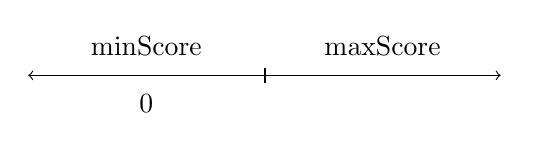
\begin{tikzpicture}[]
    \draw[<-] (0,0) -- (1.5,0);
    \draw[{[-}] (1.5,0) node[label=above:{minScore}] {} -- (3,0);
    \draw[{[-}] (1.5,0) node[label=below:{0}] {} -- (3,0);
    \draw[{|-]}] (3,0) node[label=below:{}] {} -- (4.5,0) node[label=above:{maxScore}] {};
    \draw[->] (4.5,0) node[label=below:{}] {} -- (6,0) node[label=below:{}] {};
\end{tikzpicture}
\caption{Rango de puntajes LCS}
Fuente: Elaboracion propia.
\label{intervalLCS}
\end{figure}


\begin{itemize}
  \item El puntaje más alto que se puede obtener es $\id{maxScore} = \proc{max}(|A|,|B|)$. Este puntaje representa que ambas cadenas son exactamente iguales y no se utilizaron operaciones para transformar \id{A} en \id{B}.
  \item El puntaje más bajo que se puede obtener es $\id{minScore} = 0$. Este puntaje representa que ambas cadenas son distintas y se utilizaron varias operaciones para transformar \id{A} en \id{B}.
\end{itemize}

\section{La distancia de Levenshtein}
La distancia de Levenshtein tambien es llamada distancia de edicion. Apartir de las definiciones de \cite{Cormen2009} y \cite{Halim2019}, podemos definir la distancia de Levenshtein. Dadas dos cadenas $A=[1 \twodots m]$ y $B=[1 \twodots n]$ y un conjunto de operaciones de transformacion y sus costos, donde las operaciones consisten en insertar, eliminar y reemplazar elementos de las cadenas. La distancia de Levenshtein de $A$ y $B$ es el minimo costo de operaciones que transforma $A$ en $B$. Los costos de las operaciones de transformacion son las siguientes:
\begin{enumerate}
  \item Si los caracteres $A[i]$ y $B[j]$ coinciden, entonces no se realizan operaciones se puntua $0$.
  \item Si los caracteres $A[i]$ y $B[j]$ no coinciden, se realiza la operacion de reemplazar $A[i]$ con $B[j]$, la operacion puntua $+1$.
  \item Si se realiza la operacion de insertar un caracter en $A[i]$, la operacion puntua $+1$.
  \item Si se realiza la operacion de eliminar un caracter en $A[i]$, la operacion puntua $+1$.
\end{enumerate}

Se define a $\proc{Lev}(i, j)$ como la puntuacion de la alineacion optima, para los prefijos $A[1 \twodots i]$ y $B[1 \twodots j]$. Donde sus casos base y sus Recurrencias son las siguientes:

\noindent Casos base.
\begin{itemize}
  \item $Lev(0,0) = 0$, dos cadenas vacias no puntuan.
  \item $Lev(i,0) = i$, eliminar la subcadena $A[1 \twodots i]$ para realizar la alineacion, $i>0$.
  \item $Lev(0,j) = j$, insertar un caracter en $B[1 \twodots j]$ para realizar la alineacion $j>0$.
\end{itemize}
\noindent Recurrencias para $i, j > 0$.
\begin{itemize}
  \item $Lev(i,j) = \proc{min}(opcion1, opcion2, opcion3)$
  \begin{itemize}
    \item $\id{opcion1} = Lev(i-1,j-1)$, si $A[i]$ y $B[j]$ coinciden.
    \item $\id{opcion1} = Lev(i-1,j-1) + 1$, si $A[i]$ y $B[j]$ no coinciden.
    \item $\id{opcion2} = Lev(i-1,j) + 1$, eliminar $A_i$.
    \item $\id{opcion3} = Lev(i,j - 1) + 1$, insertar $B_j$.
  \end{itemize}
\end{itemize}

El algoritmo de programacion dinamica se concentra en tres posibilidades para el ultimo par de caracteres, probando todas las posibilidades, evitando recalcular los subproblemas superpuestos. Con una funcion de puntuacion sencilla, donde una coincidencia obtiene $0$ puntos y un reemplazamiento, insercion o eliminacion obtienen $+1$, se muestra el detalle de la alineacion de $A=``ACAATCC''$ y $B=``AGCATGC''$ en la figura \ref{tableLev}. Inicialmente solo se conocen los casos base, y se rellenan los valores fila por fila de izquierda a derecha. Para rellenar $Lev(i,j)$ donde $i , j > 0$, unicamente se necesita de tres valores: $Lev(i-1,j-1)$, $Lev(i-1,j)$ y $Lev(i,j-1)$. La puntuacion de la alineacion maxima se almacena en la celda inferior derecha.
\begin{figure}[!h]
\centering
\begin{tabular}{ccccccccc}
                       & 0                      & 1                      & 2                      & 3                      & 4                      & 5                      & 6                      & 7                      \\ \cline{2-9}
\multicolumn{1}{c|}{0} & \multicolumn{1}{c|}{0} & \multicolumn{1}{c|}{1} & \multicolumn{1}{c|}{2} & \multicolumn{1}{c|}{3} & \multicolumn{1}{c|}{4} & \multicolumn{1}{c|}{5} & \multicolumn{1}{c|}{6} & \multicolumn{1}{c|}{7} \\ \cline{2-9}
\multicolumn{1}{c|}{1} & \multicolumn{1}{c|}{1} & \multicolumn{1}{c|}{0} & \multicolumn{1}{c|}{1} & \multicolumn{1}{c|}{2} & \multicolumn{1}{c|}{3} & \multicolumn{1}{c|}{4} & \multicolumn{1}{c|}{5} & \multicolumn{1}{c|}{6} \\ \cline{2-9}
\multicolumn{1}{c|}{2} & \multicolumn{1}{c|}{2} & \multicolumn{1}{c|}{1} & \multicolumn{1}{c|}{1} & \multicolumn{1}{c|}{1} & \multicolumn{1}{c|}{2} & \multicolumn{1}{c|}{3} & \multicolumn{1}{c|}{4} & \multicolumn{1}{c|}{5} \\ \cline{2-9}
\multicolumn{1}{c|}{3} & \multicolumn{1}{c|}{3} & \multicolumn{1}{c|}{2} & \multicolumn{1}{c|}{2} & \multicolumn{1}{c|}{2} & \multicolumn{1}{c|}{1} & \multicolumn{1}{c|}{2} & \multicolumn{1}{c|}{3} & \multicolumn{1}{c|}{4} \\ \cline{2-9}
\multicolumn{1}{c|}{4} & \multicolumn{1}{c|}{4} & \multicolumn{1}{c|}{3} & \multicolumn{1}{c|}{3} & \multicolumn{1}{c|}{3} & \multicolumn{1}{c|}{2} & \multicolumn{1}{c|}{2} & \multicolumn{1}{c|}{3} & \multicolumn{1}{c|}{4} \\ \cline{2-9}
\multicolumn{1}{c|}{5} & \multicolumn{1}{c|}{5} & \multicolumn{1}{c|}{4} & \multicolumn{1}{c|}{4} & \multicolumn{1}{c|}{4} & \multicolumn{1}{c|}{3} & \multicolumn{1}{c|}{2} & \multicolumn{1}{c|}{3} & \multicolumn{1}{c|}{4} \\ \cline{2-9}
\multicolumn{1}{c|}{6} & \multicolumn{1}{c|}{6} & \multicolumn{1}{c|}{5} & \multicolumn{1}{c|}{5} & \multicolumn{1}{c|}{4} & \multicolumn{1}{c|}{4} & \multicolumn{1}{c|}{3} & \multicolumn{1}{c|}{3} & \multicolumn{1}{c|}{3} \\ \cline{2-9}
\multicolumn{1}{c|}{7} & \multicolumn{1}{c|}{7} & \multicolumn{1}{c|}{6} & \multicolumn{1}{c|}{6} & \multicolumn{1}{c|}{5} & \multicolumn{1}{c|}{5} & \multicolumn{1}{c|}{4} & \multicolumn{1}{c|}{4} & \multicolumn{1}{c|}{3} \\ \cline{2-9}
\end{tabular}
\caption{Ejemplo del algoritmo de Levenshtein}
Ejemplo: A=``ACAATCC'' y B=``AGCATGC'', la puntuación de la alineación es igual a 3. \\Fuente: \cite{Halim2019}.
\label{tableLev}
\end{figure}


\subsection{Implementacion del procedimiento}
En $\proc{Levenshtein}(A,B)$ se tiene la implementación en pseudocódigo del algoritmo.
\begin{codebox}
\Procname{$\proc{Levenshtein}(A,B)$}
\li $\id{m} \gets A.length + 1$
\li $\id{n} \gets B.length + 1$
\li let $t[0 \twodots m, 0 \twodots n]$ be new table
\li \For $i \gets 0$ \To $m$ \Do
\li $t[i][0] \gets i$ \End
\li \For $i \gets 0$ \To $n$ \Do
\li $t[0][i] \gets i$ \End
\li \For $i \gets 1$ \To $m$ \Do
\li \For $j \gets 1$ \To $n$ \Do
\li \If $A[i-1] \isequal B[j-1]$ \Then
\li $t[i][j] \gets t[i - 1][j - 1]$
\li \Else
\li $t[i][j] \gets t[i - 1][j - 1] + 1$ \End
\li $t[i][j] \gets \proc{min}(t[i][j],t[i-1][j]+1)$
\li $t[i][j] \gets \proc{min}(t[i][j],t[i][j-1]+1)$ \End \End
\li \Return $t[m - 1][n - 1]$
\end{codebox}

La complejidad espacial de este algoritmo de DP es $O(n * m)$ dado que la tabla tiene dimension $n * m$. El rellenado de una celda tiene complejidad temporal de $O(1)$ por lo tanto la complejidad temporal del algoritmo es $O(n * m)$.

\subsection{Intervalo de puntajes de Levenshtein}
Los puntajes que se pueden obtener por el procedimiento $\proc{Levenshtein}$ se encuentran en el intervalo $[\id{minScore} \twodots \id{maxScore}]$. En la figura \ref{intervalLev} se muestra el intervalo.
\begin{figure}[!h]
\centering
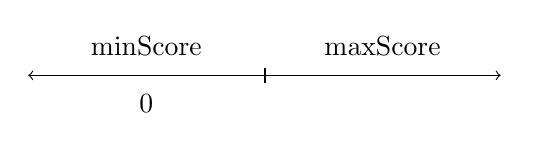
\begin{tikzpicture}[]
    \draw[<-] (0,0) -- (1.5,0);
    \draw[{[-}] (1.5,0) node[label=above:{minScore}] {} -- (3,0);
    \draw[{[-}] (1.5,0) node[label=below:{0}] {} -- (3,0);
    \draw[{|-]}] (3,0) node[label=below:{}] {} -- (4.5,0) node[label=above:{maxScore}] {};
    \draw[->] (4.5,0) node[label=below:{}] {} -- (6,0) node[label=below:{}] {};
\end{tikzpicture}
\caption{Rango de puntajes Levenshtein}
Fuente: Elaboracion propia.
\label{intervalLev}
\end{figure}

\begin{itemize}
  \item El puntaje más alto que se puede obtener es $\id{maxScore} = \proc{max}(|A|,|B|)$. Este puntaje representa que ambas cadenas son distintas y se utilizaron varias operaciones para transformar \id{A} en \id{B}.
  \item El puntaje más bajo que se puede obtener es $\id{minScore} = 0$. Este puntaje representa que ambas cadenas son exactamente iguales y no se utilizaron operaciones para transformar \id{A} en \id{B}.
\end{itemize}

\subsection{Reduccion de la complejidad espacial}
En \cite{Halim2019} explica que el truco para reducir la complejidad espacial. Durante el calculo de la solucion de cualquier subproblema solo se necesita la fila anterior y la actual. Se puede ahorrar espacio almacenando solo estas dos filas, con este truco la nueva complejidad espacial sera de $O(\proc{min}(n,m))$ colocando la cadena con menor longitud como la segunda cadena, para el ahorro de espacio. La complejidad temporal se mantiene en $O(n*m)$, la desventaja de este truco es que no puede reconstruir la solucion optima.

\subsection{Reduccion de la complejidad temporal}
En \cite{Halim2019} explica que el truco para reducir la complejidad temporal. Con el fin de reducir la complejidad temporal solo resolver los subproblemas que estan adyacentes la diagonal principal de la tabla, a una distancia \id{d}, con este truco la nueva complejidad temporal sera de $O(m * d)$, la desventaja de este truco es que no siempre se llega a obtener la alineacion óptima. Para asegurarse de obtener la solucion optima \id{d} debe ser igual \id{n}.

\section{Hashing de cadenas}
Los algoritmos de hashing ayudan a resolver un monton de problemas, uno de esos problemas consiste en la comparación de dos cadenas de forma eficiente. El algoritmo de fuerza bruta compara las cadenas caracter por caracter, esto tiene como complejidad temporal $O(\proc{min}(n,m))$ donde n y m son longitudes de las dos cadenas. El hashing de cadenas consiste en asignar a cada cadena un valor entero, y comparar los valores enteros, esto reduce la complejidad temporal en $O(1)$ cuando los valores hash ya fueron calculados previamente. Los valores hash de una cadena \id{s} de longitud \id{n} se define como:
\begin{equation}
  \proc{hash}(s) = \sum_{i=0}^{n-1}{s[i]*p^i \id{mod} \id{m}}
\label{hashValue}
\end{equation}

los valores \id{p} y \id{m} de la ecuacion \ref{hashValue} son numeros enteros positivos, donde el numero \id{p} es primo y el numero \id{m} es un valor lo suficientemente grande, con el fin de evitar colisiones. Una colision sucede cuando $\proc{hash}(s)=\proc{hash}(t)$ donde $s \neq t$.

En $\proc{compute-hash}$ se tiene la implementacion en pseudocódigo del algoritmo para calcular el hashing de cadenas.
\begin{codebox}
\Procname{$\proc{compute-hash}(s)$}
\li $p \gets 31$
\li $m \gets 10^9 + 9$
\li $\id{hash-value} \gets 0$
\li $p-pow \gets 1$
\For each $s_i \in s$ \Do
\li $\id{hash-value} \gets ((\id{hash-value} + s_i) * \id{p-pow}) \% m$
\li $p-pow \gets (\id{p-pow} * p) \% m$
\li \Return $\id{hash-value}$
\end{codebox}

